\documentclass[letterpaper,superscriptaddress,showkeys,longbibliography]{revtex4-1}\usepackage{graphicx, color}
%% maxwidth is the original width if it is less than linewidth
%% otherwise use linewidth (to make sure the graphics do not exceed the margin)
\makeatletter
\def\maxwidth{ %
  \ifdim\Gin@nat@width>\linewidth
    \linewidth
  \else
    \Gin@nat@width
  \fi
}
\makeatother

\IfFileExists{upquote.sty}{\usepackage{upquote}}{}
\definecolor{fgcolor}{rgb}{0.2, 0.2, 0.2}
\newcommand{\hlnumber}[1]{\textcolor[rgb]{0,0,0}{#1}}%
\newcommand{\hlfunctioncall}[1]{\textcolor[rgb]{0.501960784313725,0,0.329411764705882}{\textbf{#1}}}%
\newcommand{\hlstring}[1]{\textcolor[rgb]{0.6,0.6,1}{#1}}%
\newcommand{\hlkeyword}[1]{\textcolor[rgb]{0,0,0}{\textbf{#1}}}%
\newcommand{\hlargument}[1]{\textcolor[rgb]{0.690196078431373,0.250980392156863,0.0196078431372549}{#1}}%
\newcommand{\hlcomment}[1]{\textcolor[rgb]{0.180392156862745,0.6,0.341176470588235}{#1}}%
\newcommand{\hlroxygencomment}[1]{\textcolor[rgb]{0.43921568627451,0.47843137254902,0.701960784313725}{#1}}%
\newcommand{\hlformalargs}[1]{\textcolor[rgb]{0.690196078431373,0.250980392156863,0.0196078431372549}{#1}}%
\newcommand{\hleqformalargs}[1]{\textcolor[rgb]{0.690196078431373,0.250980392156863,0.0196078431372549}{#1}}%
\newcommand{\hlassignement}[1]{\textcolor[rgb]{0,0,0}{\textbf{#1}}}%
\newcommand{\hlpackage}[1]{\textcolor[rgb]{0.588235294117647,0.709803921568627,0.145098039215686}{#1}}%
\newcommand{\hlslot}[1]{\textit{#1}}%
\newcommand{\hlsymbol}[1]{\textcolor[rgb]{0,0,0}{#1}}%
\newcommand{\hlprompt}[1]{\textcolor[rgb]{0.2,0.2,0.2}{#1}}%

\usepackage{framed}
\makeatletter
\newenvironment{kframe}{%
 \def\at@end@of@kframe{}%
 \ifinner\ifhmode%
  \def\at@end@of@kframe{\end{minipage}}%
  \begin{minipage}{\columnwidth}%
 \fi\fi%
 \def\FrameCommand##1{\hskip\@totalleftmargin \hskip-\fboxsep
 \colorbox{shadecolor}{##1}\hskip-\fboxsep
     % There is no \\@totalrightmargin, so:
     \hskip-\linewidth \hskip-\@totalleftmargin \hskip\columnwidth}%
 \MakeFramed {\advance\hsize-\width
   \@totalleftmargin\z@ \linewidth\hsize
   \@setminipage}}%
 {\par\unskip\endMakeFramed%
 \at@end@of@kframe}
\makeatother

\definecolor{shadecolor}{rgb}{.97, .97, .97}
\definecolor{messagecolor}{rgb}{0, 0, 0}
\definecolor{warningcolor}{rgb}{1, 0, 1}
\definecolor{errorcolor}{rgb}{1, 0, 0}
\newenvironment{knitrout}{}{} % an empty environment to be redefined in TeX

\usepackage{alltt}
\usepackage[utf8]{inputenc}
\usepackage{color,dcolumn,graphicx,hyperref}
\usepackage{natbib}
\usepackage{footnote}
\usepackage{threeparttable}
\usepackage{scrextend}
\usepackage{setspace}
\usepackage[margin=1in]{geometry}

% stuff for coloring rows in tables - BEGIN
\usepackage{booktabs}% http://ctan.org/pkg/booktabs
\usepackage{colortbl}% http://ctan.org/pkg/colortbl
\usepackage{amsmath}% http://ctan.org/pkg/amsmath
\usepackage{xcolor}% http://ctan.org/pkg/xcolor
\usepackage{graphicx}% http://ctan.org/pkg/graphicx

\colorlet{tableheadcolor}{gray!25} % Table header colour = 25% gray
\newcommand{\headcol}{\rowcolor{tableheadcolor}} %
\colorlet{tablerowcolor}{gray!10} % Table row separator colour = 10% gray
\newcommand{\rowcol}{\rowcolor{tablerowcolor}} %
    % Command \topline consists of a (slightly modified) \toprule followed by a \heavyrule rule of colour tableheadcolor (hence, 2 separate rules)
\newcommand{\topline}{\arrayrulecolor{black}\specialrule{0.1em}{\abovetopsep}{0pt}%
            \arrayrulecolor{tableheadcolor}\specialrule{\belowrulesep}{0pt}{0pt}%
            \arrayrulecolor{black}}
    % Command \midline consists of 3 rules (top colour tableheadcolor, middle colour black, bottom colour white)
\newcommand{\midline}{\arrayrulecolor{tableheadcolor}\specialrule{\aboverulesep}{0pt}{0pt}%
            \arrayrulecolor{black}\specialrule{\lightrulewidth}{0pt}{0pt}%
            \arrayrulecolor{white}\specialrule{\belowrulesep}{0pt}{0pt}%
            \arrayrulecolor{black}}
    % Command \rowmidlinecw consists of 3 rules (top colour tablerowcolor, middle colour black, bottom colour white)
\newcommand{\rowmidlinecw}{\arrayrulecolor{tablerowcolor}\specialrule{\aboverulesep}{0pt}{0pt}%
            \arrayrulecolor{black}\specialrule{\lightrulewidth}{0pt}{0pt}%
            \arrayrulecolor{white}\specialrule{\belowrulesep}{0pt}{0pt}%
            \arrayrulecolor{black}}
    % Command \rowmidlinewc consists of 3 rules (top colour white, middle colour black, bottom colour tablerowcolor)
\newcommand{\rowmidlinewc}{\arrayrulecolor{white}\specialrule{\aboverulesep}{0pt}{0pt}%
            \arrayrulecolor{black}\specialrule{\lightrulewidth}{0pt}{0pt}%
            \arrayrulecolor{tablerowcolor}\specialrule{\belowrulesep}{0pt}{0pt}%
            \arrayrulecolor{black}}
    % Command \rowmidlinew consists of 1 white rule
\newcommand{\rowmidlinew}{\arrayrulecolor{white}\specialrule{\aboverulesep}{0pt}{0pt}%
            \arrayrulecolor{black}}
    % Command \rowmidlinec consists of 1 tablerowcolor rule
\newcommand{\rowmidlinec}{\arrayrulecolor{tablerowcolor}\specialrule{\aboverulesep}{0pt}{0pt}%
            \arrayrulecolor{black}}
    % Command \bottomline consists of 2 rules (top colour
\newcommand{\bottomline}{\arrayrulecolor{white}\specialrule{\aboverulesep}{0pt}{0pt}%
            \arrayrulecolor{black}\specialrule{\heavyrulewidth}{0pt}{\belowbottomsep}}%
\newcommand{\bottomlinec}{\arrayrulecolor{tablerowcolor}\specialrule{\aboverulesep}{0pt}{0pt}%
            \arrayrulecolor{black}\specialrule{\heavyrulewidth}{0pt}{\belowbottomsep}}%
% stuff for coloring rows in tables - END

\newcolumntype{L}{>{\arraybackslash}m{5cm}} % creates now column type to wrap text
\newcolumntype{B}{>{\arraybackslash}m{3cm}} % creates now column type to wrap text
\newcolumntype{C}{>{\arraybackslash}m{3.5cm}} % creates now column type to wrap text

\hypersetup
{
    colorlinks = true, linkcolor = blue, citecolor = blue, urlcolor = blue,
}

\begin{document}




\setstretch{2} % double space the entire manuscript

\title{Consuming altmetrics: some observations and lessons}

\author{Scott Chamberlain}
\email[E-mail: ]{scott@ropensci.org}
\affiliation{Biology Dept., Simon Fraser University, Burnaby, BC, Canada V5B 1E1}

\keywords{altmetrics; R; sotware; API}

\maketitle

\section*{Introduction}

Altmetrics, or article level metrics, measure the impact of individual articles, or objects, usually at the object level, or the author level. This is in stark contrast to the Journal Impact Factor, which is a proprietary summation of the impact of all articles in a journal (owned and calculated by Thomson Reuters ©). Altmetrics have many advantages over journal level metrics, perhaps primarily that they give impact at the article or person level. In addition, altmetrics include far more than just citations, and provide metrics in a variety of domains, including discussion by the media (mentions in the news), discussion by the public (facebook likes, tweets), and importance to colleagues (citations). 

There are many potential uses for altmetrics. Here are a number of use cases for conusming altmetrics: 

\begin{itemize}
  \item \emph{Research}. As altmetrics rise in use and popularity, research on altmetrics themselves will inevitably become a more common use case. Some recent papers have answered the questions: How do different altmetrics relate to one another \cite{yan2011,bollen2009}? What is the role of Twitter in the lifecycle of a paper \cite{darling2013}? These questions involve collecting altmetrics in bulk from altmetrics providers, and manipulating, visualizing, and analyzing the data. This use case often requires using scripting languages (e.g., Python, Ruby, R) to consume altmetrics on a computer locally (rather than in a browser). Consuming altmetrics from this perspective is somewhat different than the use case in which a user looks at altmetrics in a web browser. This use case is the target use case on which this paper is based. 
  \item \emph{Credit}. Scholars already put altmetrics on their CV's. With the rise of altmetrics, this will become much more common, especially with initiatives like that of NSF that allows scholars to get credit for \emph{products}, not just papers - and products like datasets and videos can not be measured by citations or Journal Imapact Factors. This use case will involve scholars with a wide variety of technical skills; and will likely be made easy with tools from ImpactStory or other providers. Piwowar and Priem discuss this use case further \cite{piwowar2013power}. 
  \item \emph{Filtering}. Scholars could not possibly find relavant papers efficiently given that there are now thousands of scholarly journals. Altmetrics can be used to filter. For example, Twitter can lead you to papers that are of great interest to people who's opinion you respect.
\end{itemize}

% cutout: Altmetrics can be consumed in a variety of contexts: as static text, images, or graphs alongside a pdf or website, as a javascript widget in a website and more.  

This paper discusses altmetrics from the perspective of developing and using scripting interfaces for altmetrics. From this perspective, there are a number of considerations: where can you get altmetrics data; data standardization and consistency; putting altmetrics into context, or normalization; relavance of altmetrics; data provenance, and technical barriers.

\section*{Altmetrics data providers}

There are many publishers now presenting altmetrics alongside papers on their websites. However, these publishers do not yet provide public facing APIs (Application Programming Interface) for altmetrics data at the time of writing. There are four major entities that aggreagate and provide altmetrics data: PLoS, ImpactStory, and Altmetric, and Plum Analytics (see Table 1 for details). Plum Analytics does not have an open public facing interface or API, so will not be discussed further. There are a few other smaller scale altmetrics providers, such as CitedIn (\url{http://citedin.org/}) and ScienceCard (\url{http://sciencecard.org/}), but they will not be discussed futher here since they are relatively small. PLoS and ImpactStory have open APIs, while Altmetrics API limits API requests by hour and day, and by payed vs. non-payed accounts. PLoS provides data in JSON (JavaScript Object Notation) and XML (Extensible Metadata Language), ImpactStory in JSON only, and Altmetric in JSON and JSONP. In terms of granularity, PLoS provides much more granular data than the others, with daily, monthly and yearly totals; ImpactStory provides only total values; and Altmetric provides total values, plus incremental summaries of their proprietary Altmetric score. PLoS is a publisher, while the mission of the other two is to collect and provide altmetrics data. PLoS and ImpactStory are non-profit, while Altmetric is for-profit.

The three providers overlap in some sources of altmetrics they gather, but not all (see Appendix Table A1). The fact that there is some complementarity in sources opens the possibility that different metrics can be combined from across the different providers to get more a complete set of altmetrics. For those that are compelementary, this should be relatively easy, and we don't have to worry about data consistency. However, when they share data sources, data may not be consistent between providers for the same data source (see \emph{Data standardization and consistency} below).

One of the important aspects of altmetrics is that most of the data collected by altmetrics aggregators like ImpactStory is that they aren't creating the data themselves, but rather are collecting the data from other sources that have their own licences. Thus, data licenses for PLoS, ImpactStory, and Altmetric are generally restricted to match those of the original data provider (e.g., some data providers do not let anyone to cache data). 

Note that in discussing the three providers, we are only aware of the details of each provider that are open to the public. For example, Altmetric and Plum Analytics provide some or all of their services to paying customers, which we don't cover here. 

\begin{table}[!ht]
    \begin{threeparttable}[b]
    \caption{Details on the four largest altmetrics providers.}\label{tab:a} % title of Table
        \begin{tabular}{|l|l|l|l|l|}
            \hline
            Variable & PLoS & ImpactStory & Altmetric & Plum Analytics \\
            \hline
            Open API? & Yes & Yes & Limited\tnote{d} & No \\
            Data format & JSON,XML & JSON & JSON,JSONP & Unknown \\
            Granularity\tnote{b} & D,M,Y & T & I & Unknown \\
            API Authentication & None & API key & API key & Unknown \\
            Business type & Publisher & Altmetrics provider & Altmetrics provider & Altmetrics provider \\
            Non-profit & Yes & Yes & No & No \\
            Income based on charging & For publications & unknown & Publishers & Institutions \\
            Rate limiting & Not enforced & Not enforced\tnote{c} & 1 call/sec.\tnote{d} & Unknown \\
            Products covered & Articles & Many\tnote{e} & Articles & Many\tnote{f} \\
            Software clients & R\tnote{g} & R,Javascript\tnote{h} & R,Python\tnote{i} & Unknown \\
            \hline
        \end{tabular}
        \begin{tablenotes}
            \item[a] Payed accounts with perks
            \item[b] D: day; M: month; Y: year; T: total; I: incremental summaries
            \item[c] Note: They recommend delaying a few seconds between requests
            \item[d] Also hourly and daily limits enforced; using API key increases limits
            \item[e] articles, code, software, presentations, datasets
            \item[f] articles, code, software, presentations, datasets, books, theses, etc. (see \url{http://www.plumanalytics.com/metrics.html} for a full list)
            \item[g] \url{https://github.com/ropensci/alm}
            \item[h] R (\url{https://github.com/ropensci/rimpactstory}), Javascript (\url{https://github.com/highwire/opensource-js-ImpactStory})
            \item[i] R (\url{https://github.com/ropensci/rAltmetric}), Python (\url{https://github.com/lnielsen-cern/python-altmetric})
        \end{tablenotes}
    \end{threeparttable}
\end{table}

\section*{Data standardization and consistency}

Now that there are multiple providers for altmetrics data, data consistency is something to keep in mind. For example, PLoS, ImpactStory and Altmetric do collect altmetrics from some of the same data sources. Are the numbers they present to users the same for the same paper, or are they different due to different collection dates, data sources, or methods of collection? Each of the three providers of course has the right to collect metrics as needed for their purposes. However, as altmetrics consumers and researchers, we should have a clear understanding of the potential hazards when using altmetrics data for research or otherwise. 

I used a set of 565 DOIs for full articles from PLoS journals only - this way all three providers would have data on the papers. I collected metrics from each of the three providers for each of the 565 DOIs. However, only a subset of DOIs had data from all three providers, so the final sample size was 308. For each DOI I removed any missing values, and calculated the maximum difference between values (i.e., providers) and plotted the distribution of these maximum difference values for seven altmetrics that were shared among the providers (Fig. 1). Figure 1 shows that, at least with respect to absolute numbers, PMC metrics are very different among providers, while PLoS views (relavant only to PLoS ALM and ImpactStory) are somewhat less variable among providers. Most of the altmetrics are not very different among providers, with most values at zero, or no difference among providers. 




% \begin{figure}[!ht]
%   \centering
%   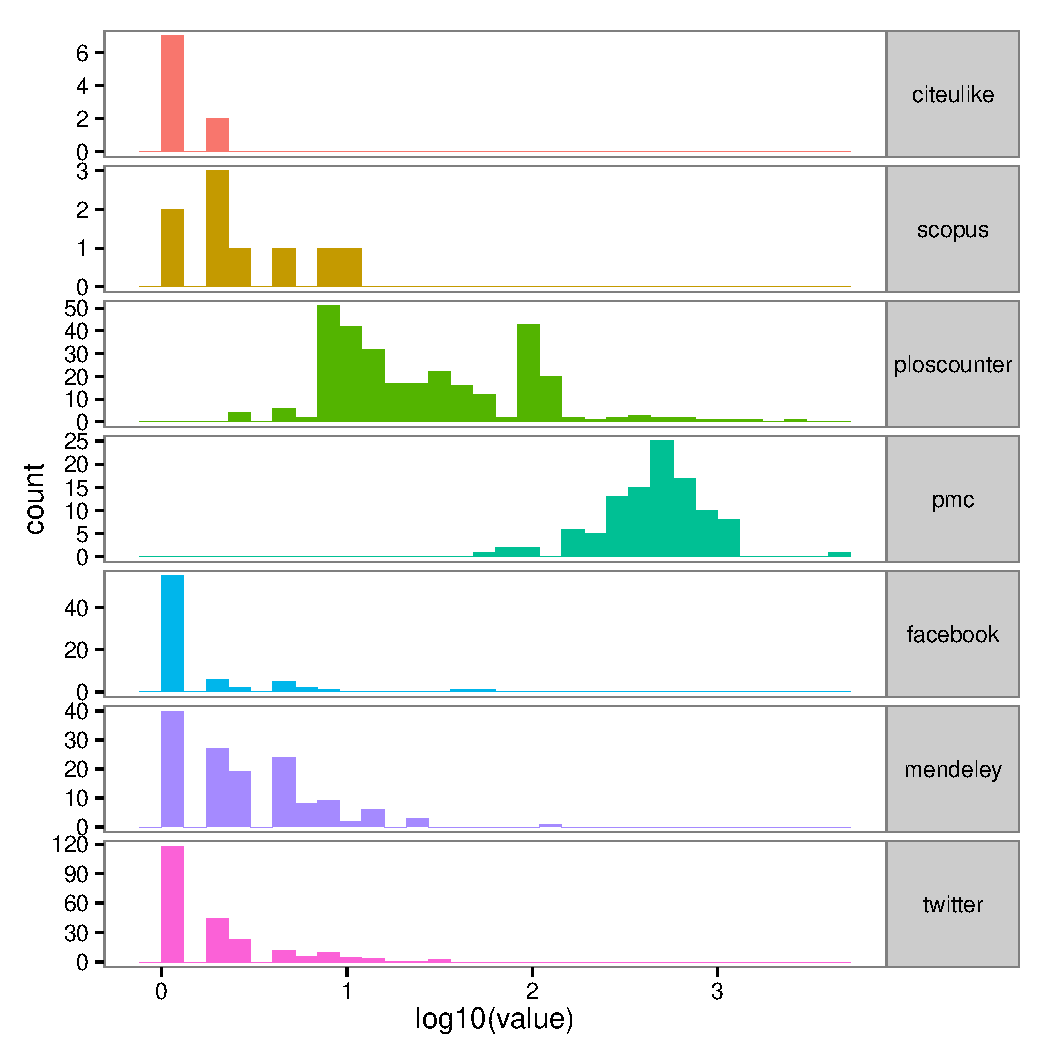
\includegraphics[width=0.7\textwidth]{figure/dataconst_plot.pdf}
%   \caption{Distribution of absolute differences in least and greatest value of each of seven different altmetrics on a set of 308 DOIs from Altmetric, ImpactStory, and PLoS ALM. Values were log10 transformed to improve comprehension.} % caption line
% \end{figure}

\begin{knitrout}
\definecolor{shadecolor}{rgb}{0.969, 0.969, 0.969}\color{fgcolor}\begin{figure}[]


{\centering 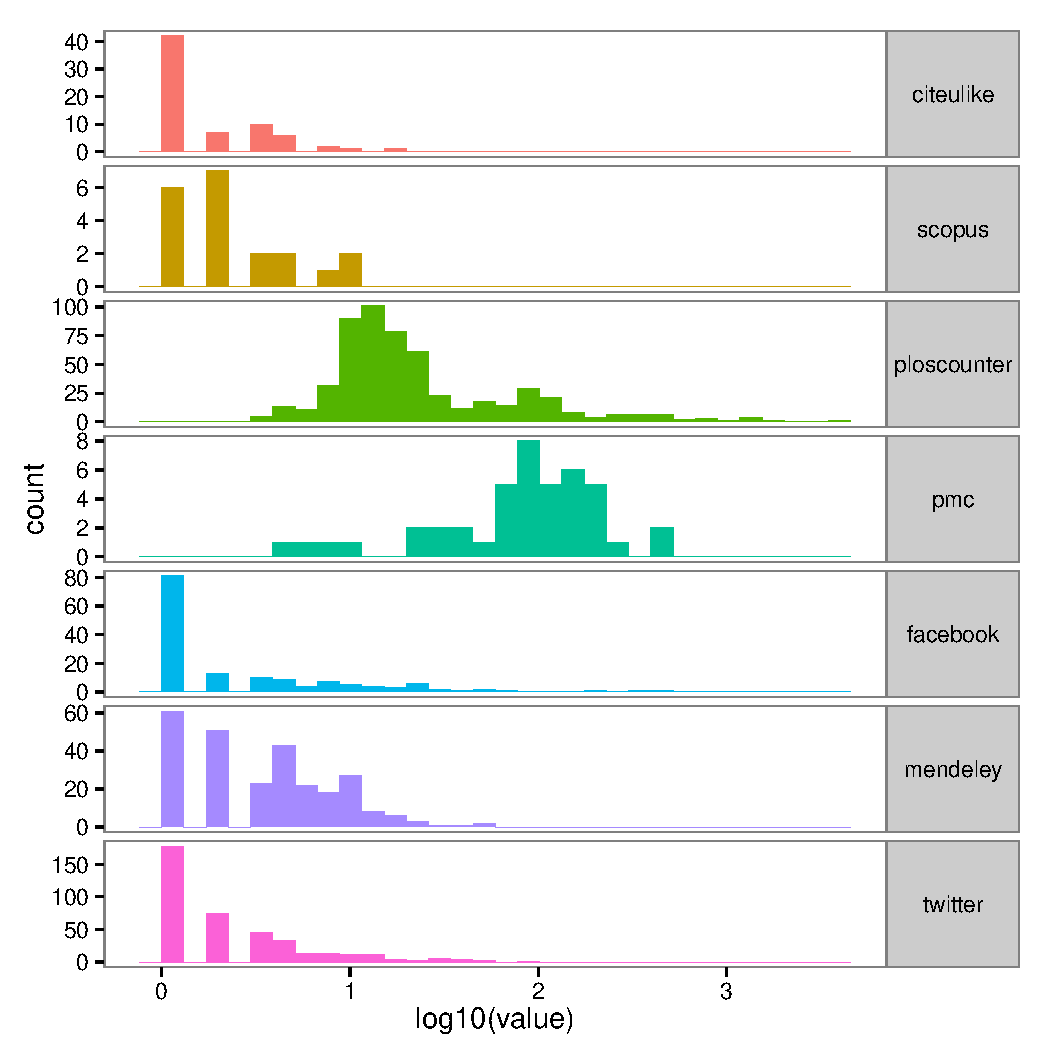
\includegraphics[width=.7\linewidth]{figure/dataconst_plot1} 

}

\caption[Distribution of absolute differences in least and greatest value of each of seven different altmetrics on a set of 565 DOIs from Altmetric, ImpactStory, and PLoS ALM]{Distribution of absolute differences in least and greatest value of each of seven different altmetrics on a set of 565 DOIs from Altmetric, ImpactStory, and PLoS ALM. Values were log10 transformed to improve visual comprehension.\label{fig:dataconst_plot1}}
\end{figure}


\end{knitrout}


What explains the differences in numbers among providers for the same metrics on the same DOIs? Numbers could differ for a number of reasons. First, data could be collected from different middle-men. For example, Twitter data is notorious for not being persistent. Thus, you either have to query the Twitter firehose constantly and store data, or go through a company like Topsy to collect tweets. Whereas ImpactStory collects tweets from Topsy, PLoS ALM and Altmetric collect tweets in an undisclosed manner. Different middle-men sources could lead to different data. Second, data could be collected at different dates. This could easily result in different data even if data are collected from the same source. This is especially obvious as ImpactStory collects some metrics via the PLoS ALM API, so those metrics that ImpactStory has from the PLoS ALM API should be the same as those that PLoS has. Fortunately, date is supplied in the returned data for all providers. Thus, I examined whether or not date could explain differences in metrics from the different providers. Figure 2 shows that there are definitely some large differences in values that could be due differences in date the data was collected, but this is not always the case (i.e., there are a lot of large difference values with very small difference in dates). 

\begin{knitrout}
\definecolor{shadecolor}{rgb}{0.969, 0.969, 0.969}\color{fgcolor}\begin{figure}[]


{\centering 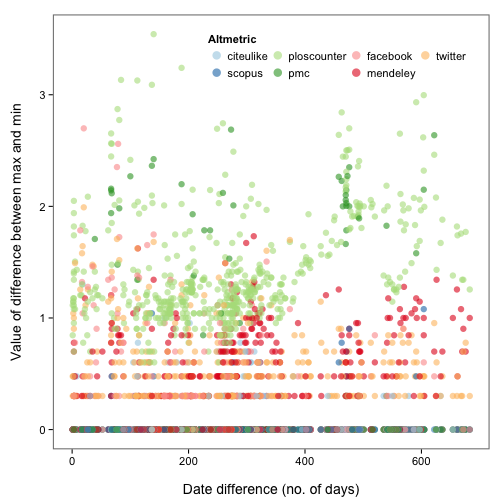
\includegraphics[width=.7\linewidth]{figure/dataconst_plot2} 

}

\caption[Distribution of absolute differences in least and greatest value of each of seven different altmetrics on a set of 565 DOIs from Altmetric, ImpactStory, and PLoS ALM]{Distribution of absolute differences in least and greatest value of each of seven different altmetrics on a set of 565 DOIs from Altmetric, ImpactStory, and PLoS ALM. Values were log10 transformed to improve visual comprehension.\label{fig:dataconst_plot2}}
\end{figure}


\end{knitrout}


That was a rough overview of hundreds of DOIs. What do the differences among providers look like in more detail? I used a set of 20 DOIs from the 565 above to show the value of each altmetric from each of the altmetrics providers for each of the 20 DOIs. Note that in some cases there is very close overlap in values for the same altmetric on the same DOI across providers, but in some cases the values are very different. 

\begin{knitrout}
\definecolor{shadecolor}{rgb}{0.969, 0.969, 0.969}\color{fgcolor}\begin{figure}[]


{\centering 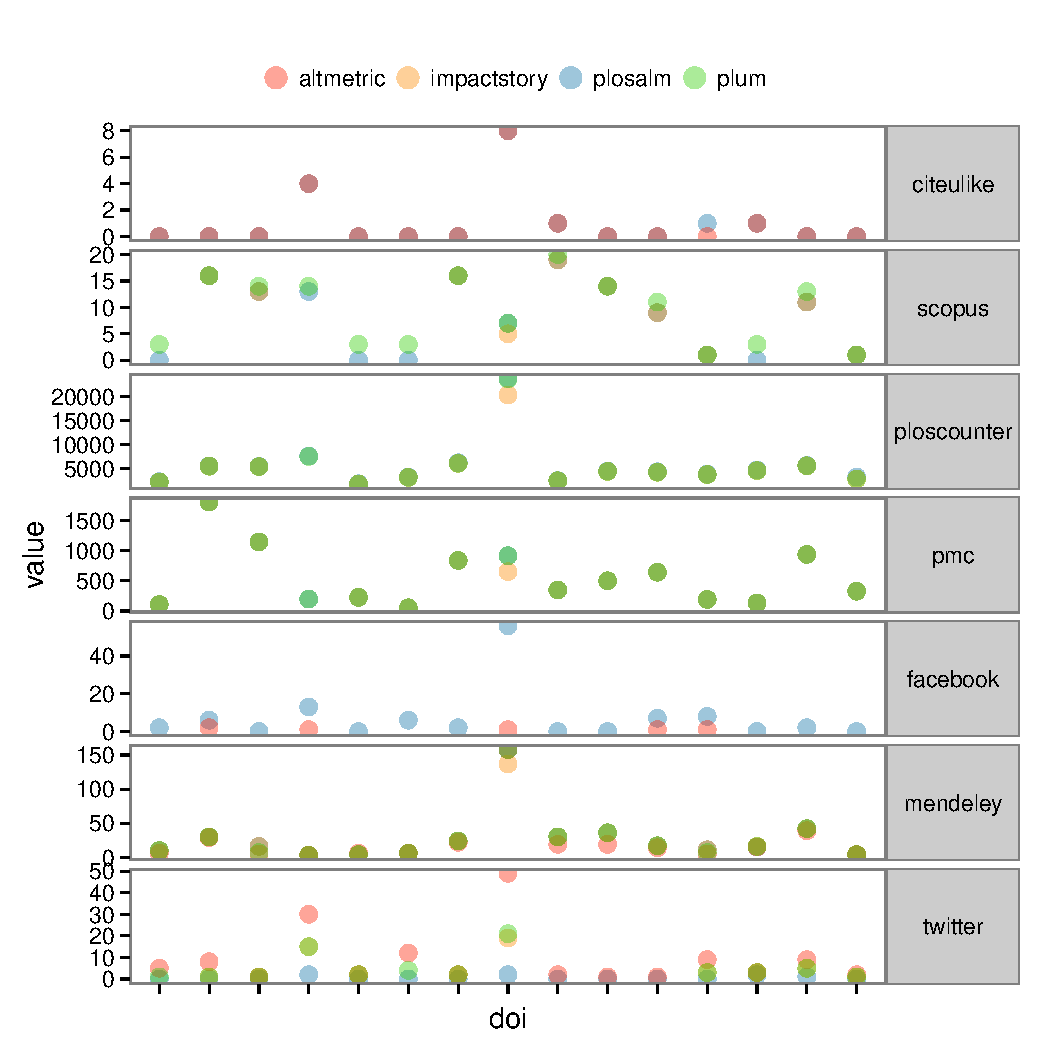
\includegraphics[width=.7\linewidth]{figure/dataconst2} 

}

\caption[A comparison of seven different altmetrics on a set of 20 DOIs from Altmetric, ImpactStory, and PLoS]{A comparison of seven different altmetrics on a set of 20 DOIs from Altmetric, ImpactStory, and PLoS. This demonstrates how altmetrics can be very similar across providers for some DOIs, but very dissimilar for others.\label{fig:dataconst2}}
\end{figure}


\end{knitrout}


An example giving what results look like may be instructive. Here is an example of calling the API of each the three providers to combine data from different sources, for the DOI \emph{10.1371/journal.pone.0018657} \cite{piwowar2011} (Table A2). In this case, only altmetrics that are shared among the providers are presented. There are many metrics that have exactly the same values among providers, though there are differences, which could be explained by the difference in the date data was collected. For example, PLoS ALM gives 6719 for combined PLoS views, while ImpactStory gives 6497 views. This is likely explained by the fact that PLoS ALM data was last updated on May 16, 2013, while ImpactStory's data was last updated on April 24, 2013. There are some oddities, however. For example, Altmetric gives 68 tweets, while ImpactStory only gives 22 tweets. ImpactStory's data was updated more recently (April 24, 2013) than that of Altmetric (November 14, 2012), which suggests something different about the way tweets among the two providers are collected as updated date alone can not explain the difference. In fact, Table A1 shows that ImpactStory collects tweets from Topsy (\url{http://topsy.com/}), while Altmetric collects them in an undisclosed manner, which obviously leads to different results.

% latex table generated in R 2.15.3 by xtable 1.7-1 package
% Tue May 21 13:02:20 2013
\begin{table}[ht]
\centering
\caption{Example of combining results across three data providers on one DOI. Note that dates that data were last modified are the same for PLoS ALM and Altmetric, but different for ImpactStory. Missing values represent data that is not given by that provider.} 
\begin{tabular}{lrrrrrrrl}
  \hline
provider & citeulike & scopus & ploscounter & pmc & facebook & mendeley & twitter & date\_modified \\ 
  \hline
plosalm & 17 & 13 & 6798 & 392 & 7 & 93 & 0 & 2013-05-21 \\ 
  altmetric & 17 &  &  &  & 1 & 92 & 71 & 2013-05-20 \\ 
  impactstory &  & 13 & 6497 & 380 &  & 91 & 22 & 2013-04-24 \\ 
   \hline
\end{tabular}
\end{table}



% \begin{figure}[!ht]
%   \centering
%   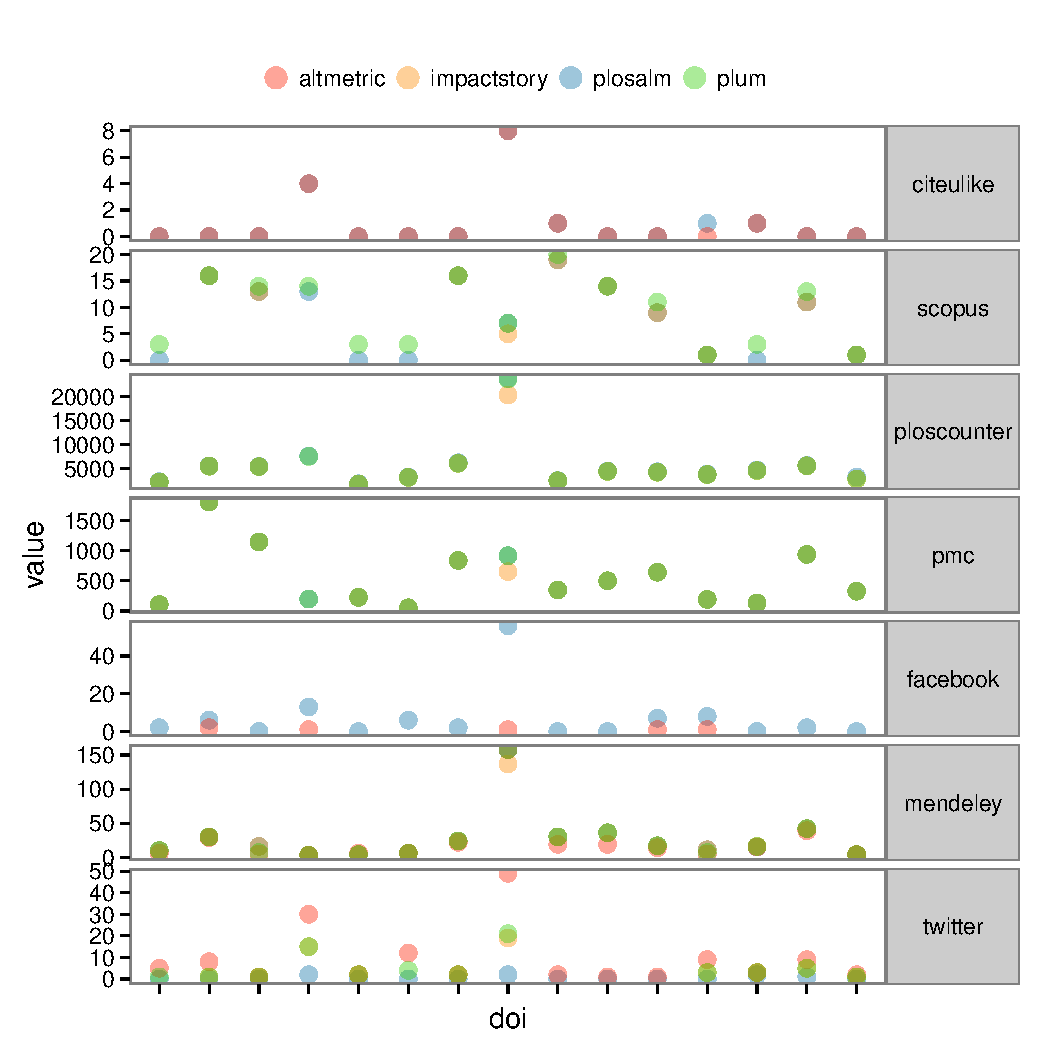
\includegraphics[width=0.7\textwidth]{figure/dataconst2.pdf}
%   \caption{A comparison of seven different altmetrics on a set of 20 DOIs from Altmetric, ImpactStory, and PLoS.} % caption line
% \end{figure}

\subsection*{A crosswalk among providers}

As discussed above, when similar data sources are collected by altmetrics providers, ideally, there would be a way to go between, for example, data from Twitter for PLoS, ImpactStory, and Altmetric. Each of the three providers of course has the right to collect metrics as needed for their purposes, but as altmetrics consumers, we should be able to compare data from the same source across providers. In Appendix Table A1, I provide a table to crosswalk metrics for the same data source among providers.

\section*{Data provenance}

Data for the same altmetrics resource could be calculated in different ways and collected at different times for the same object. The three providers already provide the date the metrics were updated. However, there is little information available, via their APIs at least, regarding how data were collected, and what, if any, calculations were done on the data before providing the data. The for-profit providers, Altmetric and Plum Analytics, especially have no obligation to share these, but the altmetrics community overall would benefit from transparency in how data are collected. 

A good step in the right direction is that ImpactStory provides a field named \emph{provenance\_url} with each metric data source. For example, for a recent paper \cite{piwowar2007}, a GET call to the ImpactStory API returns many metrics, one of which is 10 bookmarks on Delicious. Importantly, they also return the field \emph{provenance\_url}, in this case \url{http://www.delicious.com/url/9df9c6e819aa21a0e81ff8c6f4a52029}, which takes you directly to the human readble page on Delicous from where the data was collected. This is important for researchers as ideally all of our research is replicable. A nice bit about digital data such as altmetrics is that we can trace back final altmetrics from providers such as ImpactStory to their original source.

The PLoS ALM API provides something less obvious with respect to provenance, a field called \emph{events\_url}, which for the same paper above \cite{piwowar2007} returns 82 bookmarks on Citeulike, and the human readable link to where the data was collected \url{http://www.citeulike.org/doi/10.1371/journal.pone.0000308}. 

Plum Analytics does something interesting with respect to provencance - in addition to the cononical URL, they collect alias URLs for each object that they collect metrics on. For example, for the DOI \emph{10.1371/journal.pone.0018657}, they collect many URLs that point to that paper. This makes sense as a digital product is inevitably going to end up living at more than one URL, so collecting URL aliases is a good step forward for altmetrics. 

What is ideal with respect to data provenance? Is the link to where the original data was collected enough? Probably so, if no calculations were done on the original data before reaching users. However, some of the providers do give numbers which have been calculated. For example, ImpactStory puts some metrics into context by calculating a percentage relative to a reference set. Ideally, how this is done should be very clear, and replicable. 

On a related note to provenance, historical data is often helpful in a research context, for example, to know the change in a metric, rather than the point value at a certain date. PLoS provides historical altmetrics data on all their metrics, while Altmetric provides only historical data on their Altmetric score (see below section \emph{Putting altmetrics in context}), and ImpactStory does not provide historical data. Of course, historical data, especially as more and more products are tracked, may become expensive to store, so perhaps won't be emphasized by altmetrics providers. In addition, a technical barrier comes in to play in that pushing a lot of data via an API call can get very time consuming. 

\section*{Putting altmetrics in context}

Raw altmetrics data can be number of tweets, or number of html views on a publishers website. What do these numbers mean? How does the paper or dataset I care about compare to others? ImpactStory gives context to their scores by classifying scores along two dimensions: audience (scholars or public) and type of engagement (view, discuss, save, cite, recommend). Users can then determine whether a product (paper, dataset, etc.) was highly viewed, discussed, saved, cited, or recommended, and by scientists, or by the public. This abstracts away many details; however, users can drill down to the underlying data via their API and web interface.  Altmetric has a different approach. They provide context for only one metric, the altmetric score. This is a single aggregate metric, the calculation of which is not known. They do provide context for the altmetric score, including how it compares to a) all articles in the same journal, b) all articles in the same journal published within three weeks of the article, c) all articles in the Almetric database, and d) all articles in the Almetric database published within three weeks of the article. No context is given though for individual altmetrics (e.g., tweets). 

Future work should consider further dimensions of context. For example, perhaps users should be able to decide how to put their metrics into context - instead of getting raw values and values relative to a pre-chosen reference set, users could choose what reference they want to use for their specific purpose.  

% \section*{Relavance of altmetrics}
% The internet has facilitated the existence of altmetrics, as measures of impact are all around us, and many are now machine readable. However, which altmetrics are % relavant? More importantly, which altmetrics are relavant to the community you care about? XXXX. [NOT SURE IT MAKES SENSE TO KEEP THIS SECTION???]

\section{Open altmetrics}

The Journal Impact Factor (JIF), based on citation counts, the predecessor in a way to altmetrics, is a closed metric, calculated by one company, the calculation of which is unknown \cite{rossner2007show}. Given that the altmetrics movement is just at its begining, it has the chance to be a more transparent endeavour. There are a number of companies and apps appearing to provide services on top of altmetrics, some of which to create profits need to protect data outputs and the details of their operations.  Regardless, I think the altmetrics community can and should provide a level of transparency and openness that will allow research on, and use of, altmetrics. Openness in altmetrics can only be good for the science. If altmetrics are transparent, conclusions from papers, hiring decisions, and more can be verified by third parties. In addition, transparent altmetrics are less likely to be gamed, as they JIF has been gamed \cite{arnold2011}. Some good steps have been made to open altmetrics by altmetrics providers themselves. For example, many conferences and meetings have occurred where altmetrics providers and other interested parties hash out issues. 

Another issue to consider in open altmetrics are the primary altmetrics sources. The difference between Twitter and App.net is a good example. Twitter makes money off advertisements and having a relatively closed system (\url{http://techonomy.com/2012/08/video-jack-dorsey-on-twitters-business-model/}). A better option, with similar data, would be App.net. App.net has a much smaller set of users relative to Twitter - however, App.net's business model is to charge users to use the service, but make the data very open. Twitter makes more money from closing down data, whereas App.net makes more money from opening up their data. There is currently a heavy dependence on Twitter in the altmetrics community. Perhaps we should think about building the scientific community on App.net where openness can thrive. 

\section*{Technical barriers to use}

Some users of altmetrics may only require basic uses of altmetrics, like including altmetrics on their CV's \cite{piwowar2013power} to show the various impacts that their research has had. Some may want to go deeper, and collect altmetrics in mass. Using altmetrics via a scripting language means that the user has to consider whether the data source is machine readable, how easy the data is to retrieve and manipulate once retrieved, and whether they have to authenticate. First, of the three altmetrics providers discussed, all provide an API, which means their data is easily machine readable. Second, how data is returned to the user can be important if the user is interacting with the API directly. Fortunately, many libraries, or extensions, exist to a number of programming languages relavant to scholars, which deal with preparing the data for easy consumption for users (see Table 1 for links to libraries). Last, authentication can be a barrier to use in that if a user has to take extra step of authenticating, they may not bother. There are a variety of possible authentication methods, some of which include: a) no authentication, b) username and password pair, c) API key, and d) OAuth (including OAuth1 and OAuth2) (Table 1). These different options make sense in different use cases. The first, no authentication, used by PLoS, makes sense when an API is first released and testers are needed to get feedback. A benefit of an API with no authentication is the barrier to entry is lower. That is, if you don't have to ask a user to register to get an API key they are more likely to use the API. The second and third options, username/password pair and API key are relatively similar; API keys are used by both ImpactStory and Altmetric (Table 1). The last option, OAuth, is not used by any of the altmetrics providers. This authentication method is however used by many API providers. From the viewpoint of a consumer in a desktop scripting language, OAuth can be painful. What works better for scripting languages are the first three options.  

\section*{Conclusion}

XXXXXX

\section*{Acknowledgments}

I thank Martin Fenner for inviting me to write a paper in this special issue on altmetrics, and for helpful feedback from Carl Boettiger, Karthik Ram, and X on earlier versions of this manuscript.
  
\section*{References}
\bibliography{refs}

\section*{Appendix A. Crosswalk among providers.}

The following Table A1 provides a crosswalk between altmetrics data collected by the three data providers. Note that these variables relate to one another across providers, but the data may be collected differently, and so for example, altmetrics collected for Twitter may differ between PLoS, ImpactStory and Altmetric. Where data sources are shared among at least two providers, I used only those fields that would give the same data if data were collected on the same date and all other things being equal. For example, PLoS ALM's field \emph{pubmed} is equivalent to ImpactStory's \emph{pubmed:pmc\_citations} field.

\begin{table}[!ht]
\begin{threeparttable}[b]
\caption{Data sources used in taxize, tasks available, and links to them}
\begin{tabular}{|B|B|L|C|}
\hline
\headcol Data source & PLoS\tnote{a} & ImpactStory\tnote{b} & Altmetric\tnote{c} \\
\hline
Biod & biod & No & No \\
\rowcol Connotea & connotea & No & No \\
General blogs & bloglines & No & No \\
\rowcol Nature blogs & nature & No & No \\
Postgenomic & postgenomic & No & No \\
\rowcol Researchblogging & researchblogging & No & No \\
WebOfScience citations & webofscience & No & No \\
\rowcol Dryad & No & dryad:total\_downloads package\_views & No \\
Figshare & No & figshare:views shares downloads & No \\
\rowcol Github & No & github:forks stars & No \\
PLoS Search & No & plossearch:mentions & No \\
\rowcol Slideshare & No & slideshare:favorites views comments downloads & No \\
Google+ & No & No & cited\_by\_gplus\_count \\
\rowcol MSM & No & No & cited\_by\_msm\_count \\
News articles & No & No & Yes \\
\rowcol Reddit & No & No & cited\_by\_rdts\_count \\
Citeulike & citeulike & citeulike:bookmarks & No \\
\rowcol Crossref & crossref & plosalm:crossref\tnote{d} & No \\
PLoS ALM & counter(pdf\_views + html\_views)\tnote{e} & plosalm(html\_views, pdf\_views) & No \\
\rowcol PMC & pmc & plosalm:pmc\_full-text + pmc\_pdf\tnote{f} & No \\
PubMed & pubmed & pubmed:pmc\_citations\tnote{g} & No \\
\rowcol Scienceseeker & scienceseeker & scienceseeker:blog\_posts & No \\
Scopus citations & scopus & plosalm:scopus\tnote{h} & No \\
\rowcol Wikipedia & wikipedia & wikipedia:mentions & No \\
Delicious & No & delicious:bookmarks & cited\_by\_delicious\_count \\
\rowcol Facebook & facebook & facebook:shares\tnote{i} & cited\_by\_fbwalls\_count \\
Mendeley readers & mendeley shares & mendeley readers\tnote{j} & mendeley readers \\
\rowcol Twitter & twitter & topsy:tweets\tnote{k} & cited\_by\_tweeters\_count \\
\hline
\end{tabular}
\begin{tablenotes}
    \item[a] These are the exact names for each data source in the PLos ALM API. For example: \url{http://alm.plos.org/api/v3/articles?ids=10.1371/journal.pone.0018657&source=twitter}.
    \item[b] You can not request a specific source from the ImpactStory API, so these are the names of the fields in the returned json. For example, see the json from this call: \url{http://api.impactstory.org/v1/item/doi/10.1371/journal.pone.0018657?key=YOURAPIKEY}.
    \item[c] You can not request a specific source from the Altmetric API, so these are the names of the fields in the returned json. For example, see the json from this call: \url{http://api.altmetric.com/v1/doi/10.1371/journal.pbio.0018657?key=YOURAPIKEY}.
    \item[d] Collected from the PLoS ALM API. 
    \item[e] PLoS ALM also provides xml\_views. 
    \item[f] Collected from the PLoS ALM API. Other PMC data fields collected from PLoS ALM (pmc\_abstract, pmc\_supp-data, pmc\_figure, pmc\_unique-ip) and from PubMed (suppdata\_views, figure\_views, unique\_ip\_views, pdf\_downloads, abstract\_views, fulltext\_views).
    \item[g] Should be equivalent to plosalm:pubmed\_central. ImpactStory also collects pubmed:pmc\_citations\_reviews f1000 pmc\_citations\_editorials.
    \item[h] Collected from the PLoS ALM API. Scopus citations also collected from Scopus itself, in the field scopus:citations.
    \item[i] ImpactStory also collects Facebook clicks, comments, and likes. 
    \item[j] ImpactStory also collects Mendeley readers by discipline, number of groups that have added the article, percent of readers by country, and percent of readers by career\_stage. 
    \item[k] ImpactStory also collects the number of influential\_tweets from Topsy.
\end{tablenotes}
\end{threeparttable}
\end{table}

\end{document}
